\chapter{\textbf{AEmilia Model}}

The model implemented by us in Aemilia is modeled in a phase prior to refactoring.

\section{Work Planning}

The workflow was:
\begin{itemize}
\item Study of theoretical concepts of Aemilia;
\item Drafting of Flow Graph;
\item Drafting of State Diagram;
\item Implementation of the Model;
\item Test and Analysis of results.
\end{itemize}

\section{Aemilia Flow Graph}

A Flow Graph represents the topology of an architecture described in AEmilia. It is convenient to start with the flow graph representation of the architectural type and then to specify the behavior of each node.  

\begin{center}
  \makebox[\textwidth]{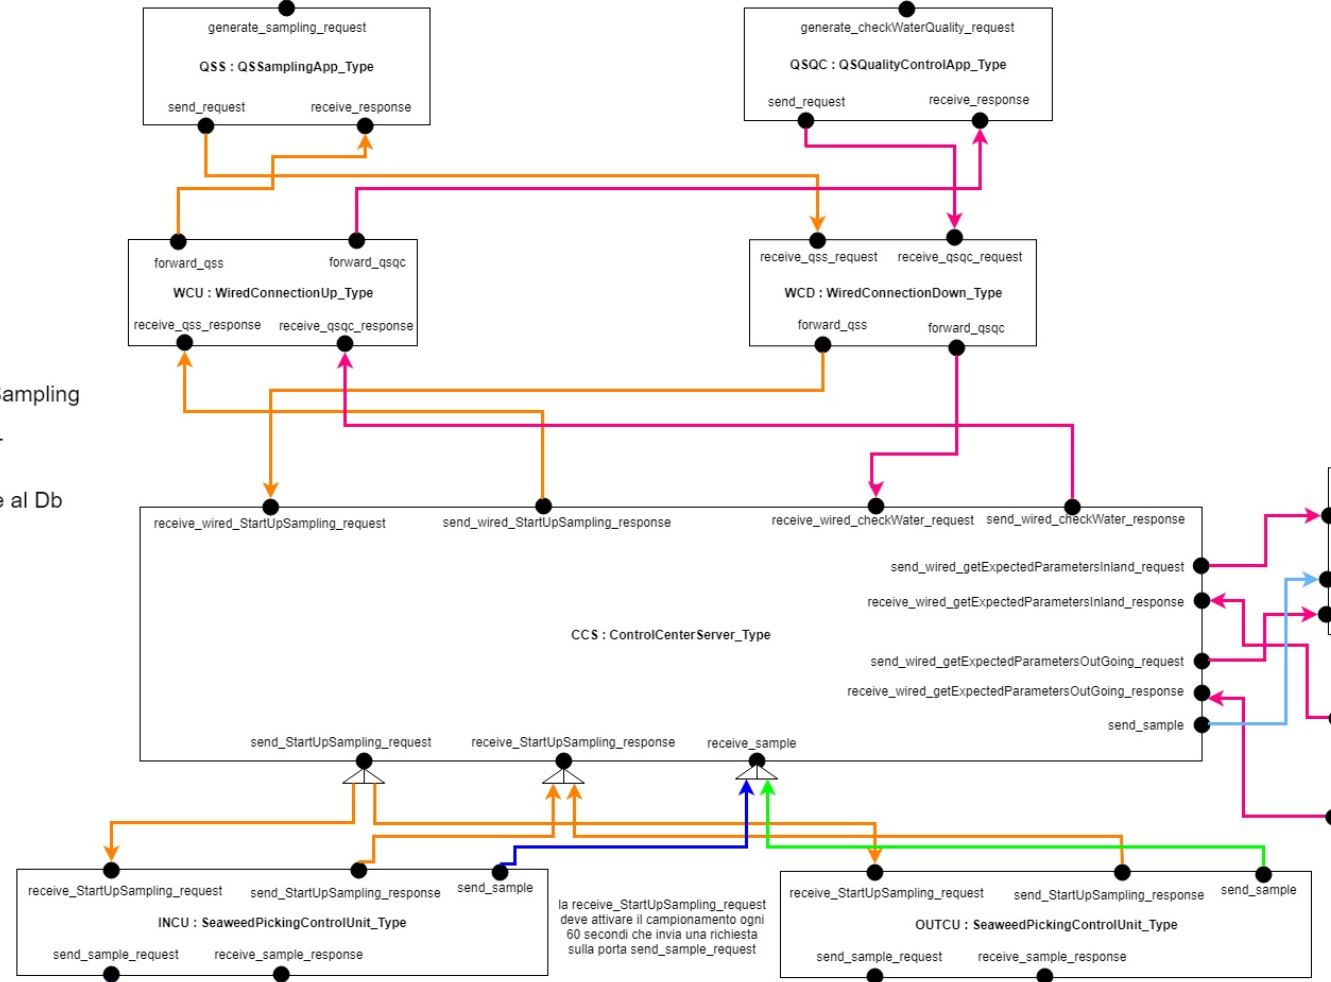
\includegraphics[width=\textwidth]{schermata1.JPG}}
\end{center}
\bigskip
\captionof{figure}{Flow Graph Extract}

\section{Aemilia State Diagram}

In describing the behavior, we created our Diagrams for each Node of the Flow Graph.

\begin{minipage}{0.3\textwidth}
\bigskip
  \makebox[\textwidth]{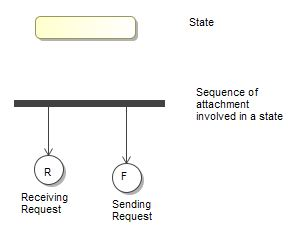
\includegraphics[width= 8cm]				{Legenda.JPG}}
\captionof{figure}{Legenda}
\end{minipage}
\hfill
\begin{minipage}{0.4\textwidth}\raggedleft
We have a block representing the state, a fork under which there is a
sequence of attachments involved within the same state, two circumferences representing these attachments
\end{minipage}
\bigskip

Below you can see an extract of it:

\begin{center}
  \makebox[\textwidth]{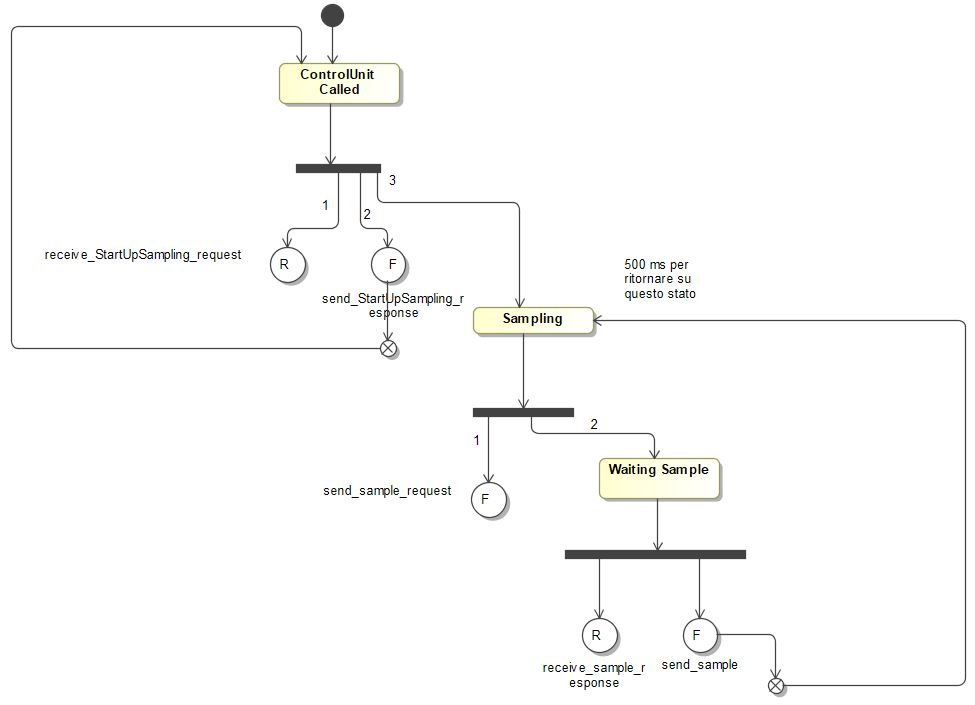
\includegraphics[width=\textwidth]				{stateDiagram.JPG}}
\end{center}
\bigskip
\captionof{figure}{State Diagram Extract}
\bigskip

In this image we see the behavior of the component "SeaweedPicking Control Unit." 


\section{Implementation Of The Model}

\subsection{Two Towers's Performance Evaluator limits}

To simulate the presence of 1000 sensors in and out we came across a variety of problems that forced us to vary the model and its implementation. The initial idea was to have in the Flow Graph 1000 instances of the Architecture Element Type "Sensor Type" incoming and outgoing, but in the next phase of the perfect evaluator Two Towers notified us that the size of the Markov Chain was too large.\\
Subsequently to overcome this limitation we thought to have a single sensor in input and output whose Delay Rate was increased by a factor open to the number of sensors in input and output that we wanted to have previously.\\
We made this choice because we thought that having only one sensor whose short wait was the closest possible to have a number of distinct sensors with a greater wait so as to stress the system in equal way.\\
Another problem encountered was that of stressing the system with the presence, as in jmt, of a population of 1000 jobs of the type of StartUp Sampling Water Inland and Outgoing. In fact, we initially tried to generate exactly 1000 StartUp messages with a buffer, but the Perfomance Evaluator in Two Towers never seemed to arrive at a solution in an acceptable time.\\
At this point we adopted the choice of having a single activation of the two StartUps aware of the fact that it was not the best choice as far from the real scenario, but compared to the simulation performed in jmt, we knew that the workload on the system of these it was not excessively large\\

\subsection{Implementation Code}

Once the behavior of the various nodes, the architecture has been written following the syntax of Aemilia. Below, we will be proposed snippets, coming from previous pictures. 

\lstset {language = C}
\bigskip
\begin{lstlisting}
ELEM_TYPE SeaweedPickingControlUnit_Type(const rate SPCU_send_StartUpSampling_response_rate, const rate SPCU_send_sample_request_rate, 
	const rate SPCU_send_sample_rate, const rate SPCU_delay_rate, const integer sensors_num)

BEHAVIOR

	ControlUnitCalled(void;void) = 
		<receive_StartUpSampling_request, _> . <send_StartUpSampling_response, exp(SPCU_send_StartUpSampling_response_rate)> . Sampling();

	Sampling(void;void) = 
		<send_sample_request, exp(SPCU_send_sample_request_rate)> . WaitingSample();

	WaitingSample(void;void) = 
		<receive_sample_response, _> . <send_sample, exp(SPCU_send_sample_rate)> . Delay();

	Delay(void;void) =
		<delay, exp(SPCU_delay_rate * sensors_num)> . Sampling()


INPUT_INTERACTIONS

	UNI receive_StartUpSampling_request;
		receive_sample_response

OUTPUT_INTERACTIONS 

	UNI send_StartUpSampling_response;
		send_sample;
		send_sample_request
\end{lstlisting}

\section{Test And Analysis Of Results}

After building the model, it was written a file describing the
performance measures to be analyzed. 

\lstset {language = C}
\bigskip
\begin{lstlisting}
MEASURE SeaweedPickingINControlUnitUtilization IS
	ENABLED(INCU.send_StartUpSampling_response) -> TRANS_REWARD(1)
	ENABLED(INCU.send_sample) -> TRANS_REWARD(1)
	ENABLED(INCU.send_sample_request) -> TRANS_REWARD(1);
\end{lstlisting}

After simulating the Model the results are this:

\lstset {language = C}
\bigskip
\begin{lstlisting}
- Value of measure "ControlCenterServerUtilization":
	0.003647

- Value of measure "WaterCompanyServerUtilization":
	0.00271904

- Value of measure "WaterCompanyDiskUtilization":
	0.00225506

- Value of measure "SeaweedPickingINControlUnitUtilization":
	0.0017911

- Value of measure "SeaweedPickingOUTControlUnitUtilization":
	0.0017911

- Value of measure "PurificationSystemServerUtilization":
	0.000463978
\end{lstlisting}

%%Controllare e modificare frase nel caso
As can be seen from the results the values obtaines from the Aemilia simulation are close to those of JMT  exept for the Water Company Disk and the non functional requirements specified at the beginning are all respected.\\

\subsection{Bottelneck Test}

In a second phase we increased the number of sensors by the same number for which we had the bottoleneck on the Water Company Disk on jmt but from the results of the simulation with Aemilia we did not have a worse use of the aforementioned node significantly so as to highlight the presence of a Bottleneck.\\
For this reason we tried to increase the number of sensors in a significant way but from the results of the simulation we noticed that the utilization of the system did not increase beyond a certain threshold and for this we assumed the presence of an asymptote.

\subsection{Another Modeling Attempt}


Not satisfied with the results of the previous simulations we have made a further model not starting from the deployment and the sequence diagram but from the queueing network. We know that this choice is wrong because we treat two different models but we wanted a comparison with the simulations performed on jmt.\\
In the image below you can see the new Flow Graph:

%%immagini Flow Graph

But also in this case the simulation results both with 1000 inland and outgoing sensors and for the number of sensors for which the bottleneck should be presented on the Water Company Disk are not comparable to those of jmt.\\

%%Immagini risultati simulazione

Against this we came to the conclusion that the subsystem we considered was not comparable between jmt and Aemilia.